\section{Durchführung}
Der Versuchsaufbau wird nach Abbildung (\ref{fig:aufbau}) aufgebaut.

\begin{figure}
            \centering
               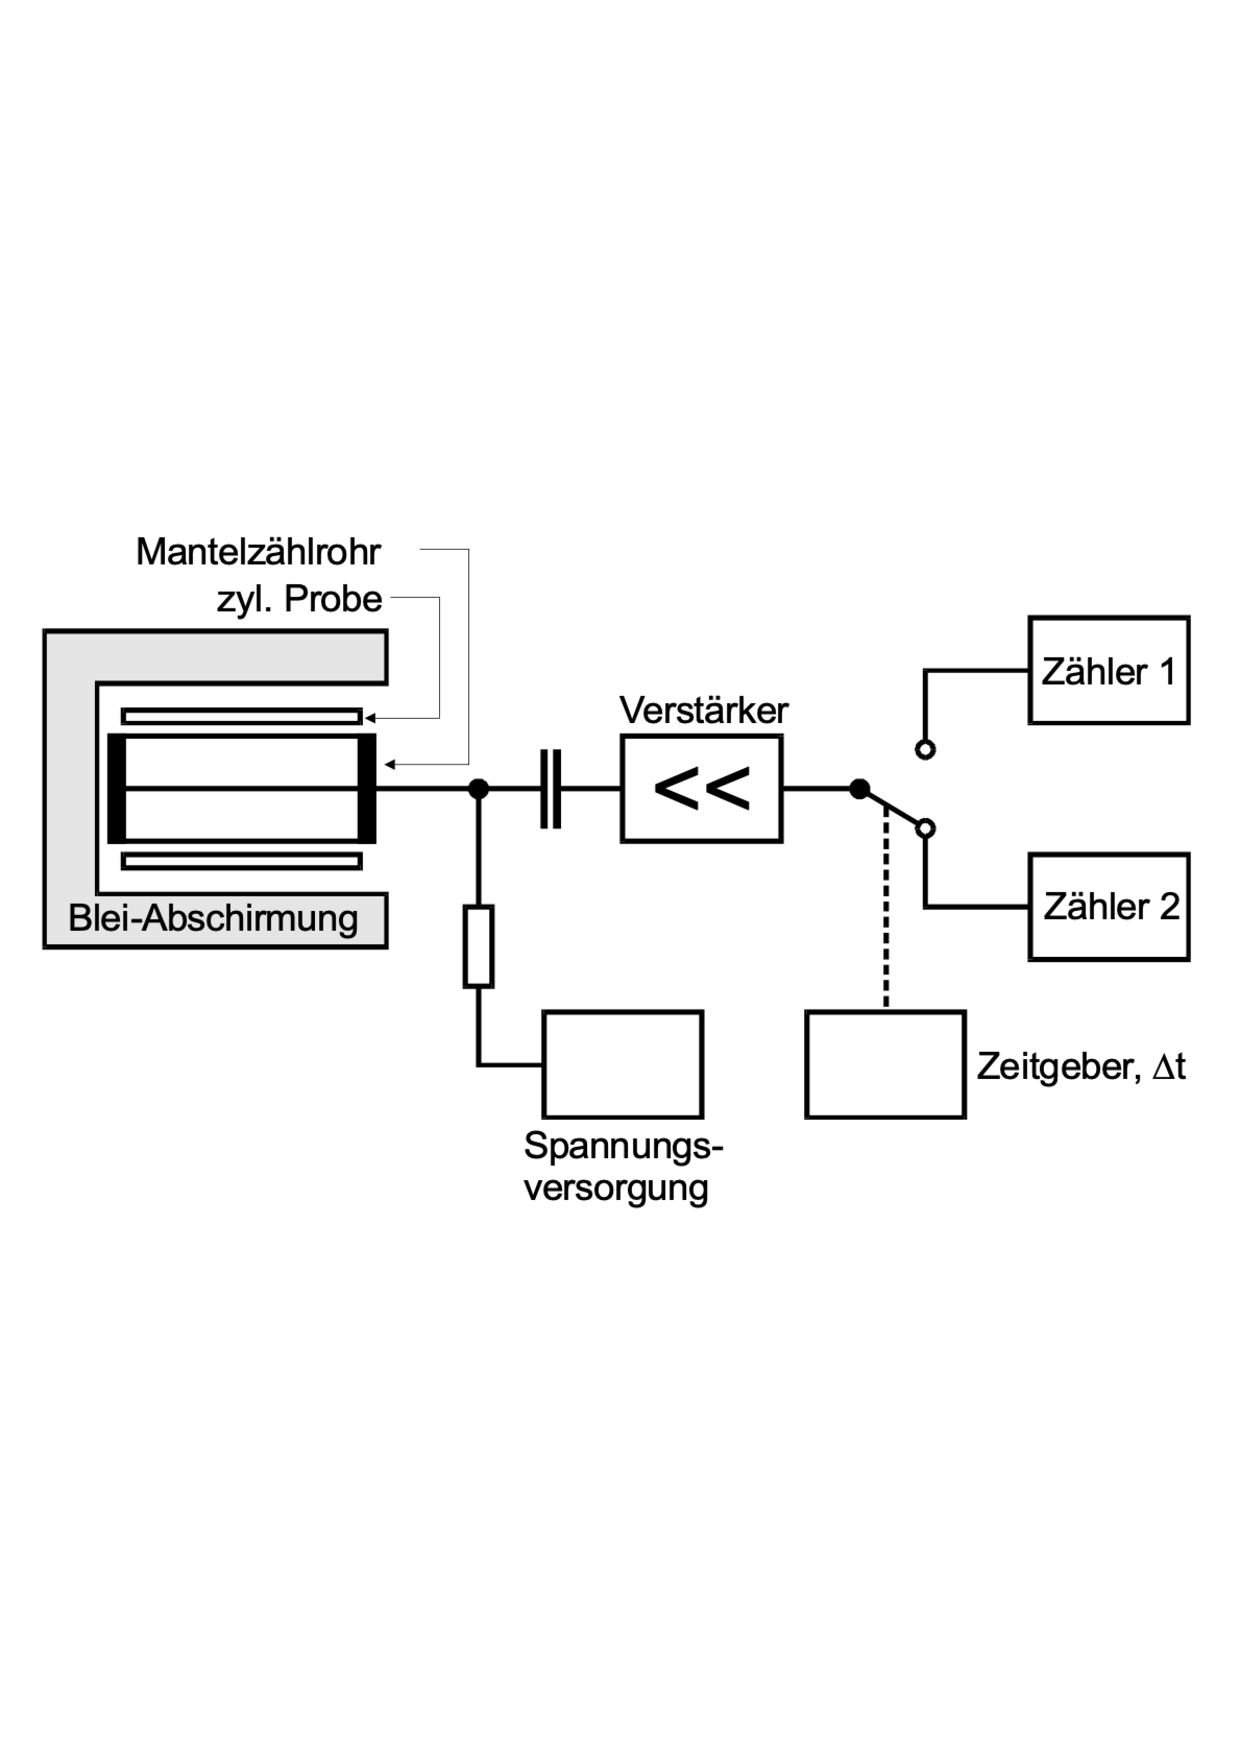
\includegraphics[height=5cm]{aufbau.pdf}
               \caption{Versuchsaufbau (Quelle: \cite{V702}).}
               \label{fig:aufbau}
\end{figure}

\subsection{Aufgabe 1)}
\noindent
Zunächst wird der Untergrund bestimmt. 
Das Messintervall wird t=300s gewählt und mit einem Codierschalter an der Frontplatte des Gerätes eingestellt.
Die Untergrundrate wird mehrfach gemessen und notiert.
In Tabelle (??) sind die gemessenen Werte aufgeführt.

\subsection{Aufgabe 2)}
\noindent
Zur Bestimmung der Halbwertszeit wird die Vanadiumprobe in der Neutronenquelle nach Abbilung %(\ref{fig:nq}) 
aktiviert und 
danach direkt auf das Geiger-Müller-Zählrohr gesteckt.
Das Messintervall wird $\Delta \text{t} = 30 \si{\second}$ gewählt und die Messung wird gestartet.
Die Messwerte werden von der Anzeige abgelesen, notiert und sind in Tabelle (??) aufgeführt.


\subsection{Aufgabe 3)}
Analog zur Halbwertszeitbestimmung von Valadium wird die Rhodiumprobe aktiviert und auf das Geiger-Müller-Zählrohr gesteckt,
wobei hier ein Messintervall von $\Delta \text{t} = 15 \si{\second}$ gewählt wird.
Die Messung wird gestartet und die Messwerte werden aufgenommen.
Diese sind in Tabelle (??) aufgeführt.